\section{Woche 4 - AK OpenSource \headerand OpenSource Forum Erfurt} \label{sec:bericht-wo-4}

% Woche 4 (2023-09-25 bis 2023-09-29)

\lweekdaymarginpar{\weekdayMondayLong}

Nach einer kurzen Nacht, in der ich die letzten Feinschliffe an meinem Präsentationsskript anwendete, besprach ich Montag mit meinem Chef noch die letzten Unklarheiten.
Eines meiner Probleme bis jetzt war ein spezifischer Teil der Präsentation, der über ein Thema ging, mit dem sich zwar mein Chef gut auskennt, ich allerdings sehr wenig.
Mein Chef übernahm glücklicherweise kurzerhand diesen Teil.
Den Rest des Tages nutzte also ich lieber im Home-Office, um in Ruhe die Präsentation zu üben und meine Reisetasche für die morgige Reise nach Erfurt zu packen.

\sweekdaymarginpar{\weekdayTuesdayLong}

Der Dienstag begann früh mit unserer Reise mit dem ICE nach Erfurt.
Während der Zugfahrt nutzten mein Chef und ich die Zeit für eine letzte Durchsprache unserer Präsentation.
Angekommen in Erfurt ging es direkt in den nahegelegenen Räumlichkeiten der DB Systel.
Dort gab es zunächst einige einleitende Worte und eine Vorstandswahl, bevor ich mit meiner Präsentation dran war.

Meine Kollegen vor Ort haben mich noch einmal ermutigt und trotz anfänglicher Nervosität verlief alles reibungslos:
Ich war gut vorbereitet, hatte die Präsentation gut geübt und die Themen, die ich vorstellte, gehören zu meinem täglichen Arbeitsbereich seit drei Jahren.
Ich brauchte mein Skript kaum und das Feedback war ausschließlich positiv, was mich sehr gefreut hat, denn ich wollte wirklich einen Mehrwert in diese Runde bringen.

Abends wurde vom {\bitkom} eine Stadtführung und ein gemeinsames Abendessen mit anderen Teilnehmern des OpenSource Forums des nächsten Tages organisiert, an welchen wir teilnahmen.
Dort, und bereits beim Arbeitskreis, konnten wir uns auch mit den anderen Teilnehmern austauschen.

\sweekdaymarginpar{\weekdayWednesdayLong}

Das OpenSource Forum der {\bitkom} bot dann eine entspannte Alternative zum vorherigen Tag, bei dem die Teilnehmer vielfältige Präsentationen verfolgen und sich untereinander auszutauschen konnten.
Besonders spannend waren die Einblicke in die Open-Source-Strategien großer Unternehmen wie SAP, Siemens und Mercedes.
Die Parallelen im Bezug auf die aktuellen Herausforderungen und Lösungsansätze für die Verwaltung von Schwachstellen und Lizenzen von Open-Source-Software in ihren Produkten und Projekten haben mich etwas überrascht und bestätigten die Relevanz unserer Arbeit.

\begin{figure}[htbp] % here, top, bottom, separate page
    \centering
    \includegraphics[width=0.5\textwidth, keepaspectratio]{res/img/2023-10-19-yan-ak-os}
    \caption{Auf dem Forum Open Source der Bitkom 2023}
    \label{fig:foss23-yan}
\end{figure}

Ein großer Programmpunkt war auch der {\bitkom} OpenSource Monitor\footnote{\url{https://www.bitkom.org/opensourcemonitor2023}}, den die {\metaeffekt} gesponsert hat und damit einen Beitrag über den Cyber Resilience Act\footnote{\url{https://digital-strategy.ec.europa.eu/en/policies/cyber-resilience-act}} in diesem verfassen durfte.
Wir wurden auch auf der großen Leinwand aufgeführt, wie in Abbildung\ \ref{fig:foss23-sponsor-metaeffekt} zu sehen ist.

\begin{figure}[htbp] % here, top, bottom, separate page
    \centering
    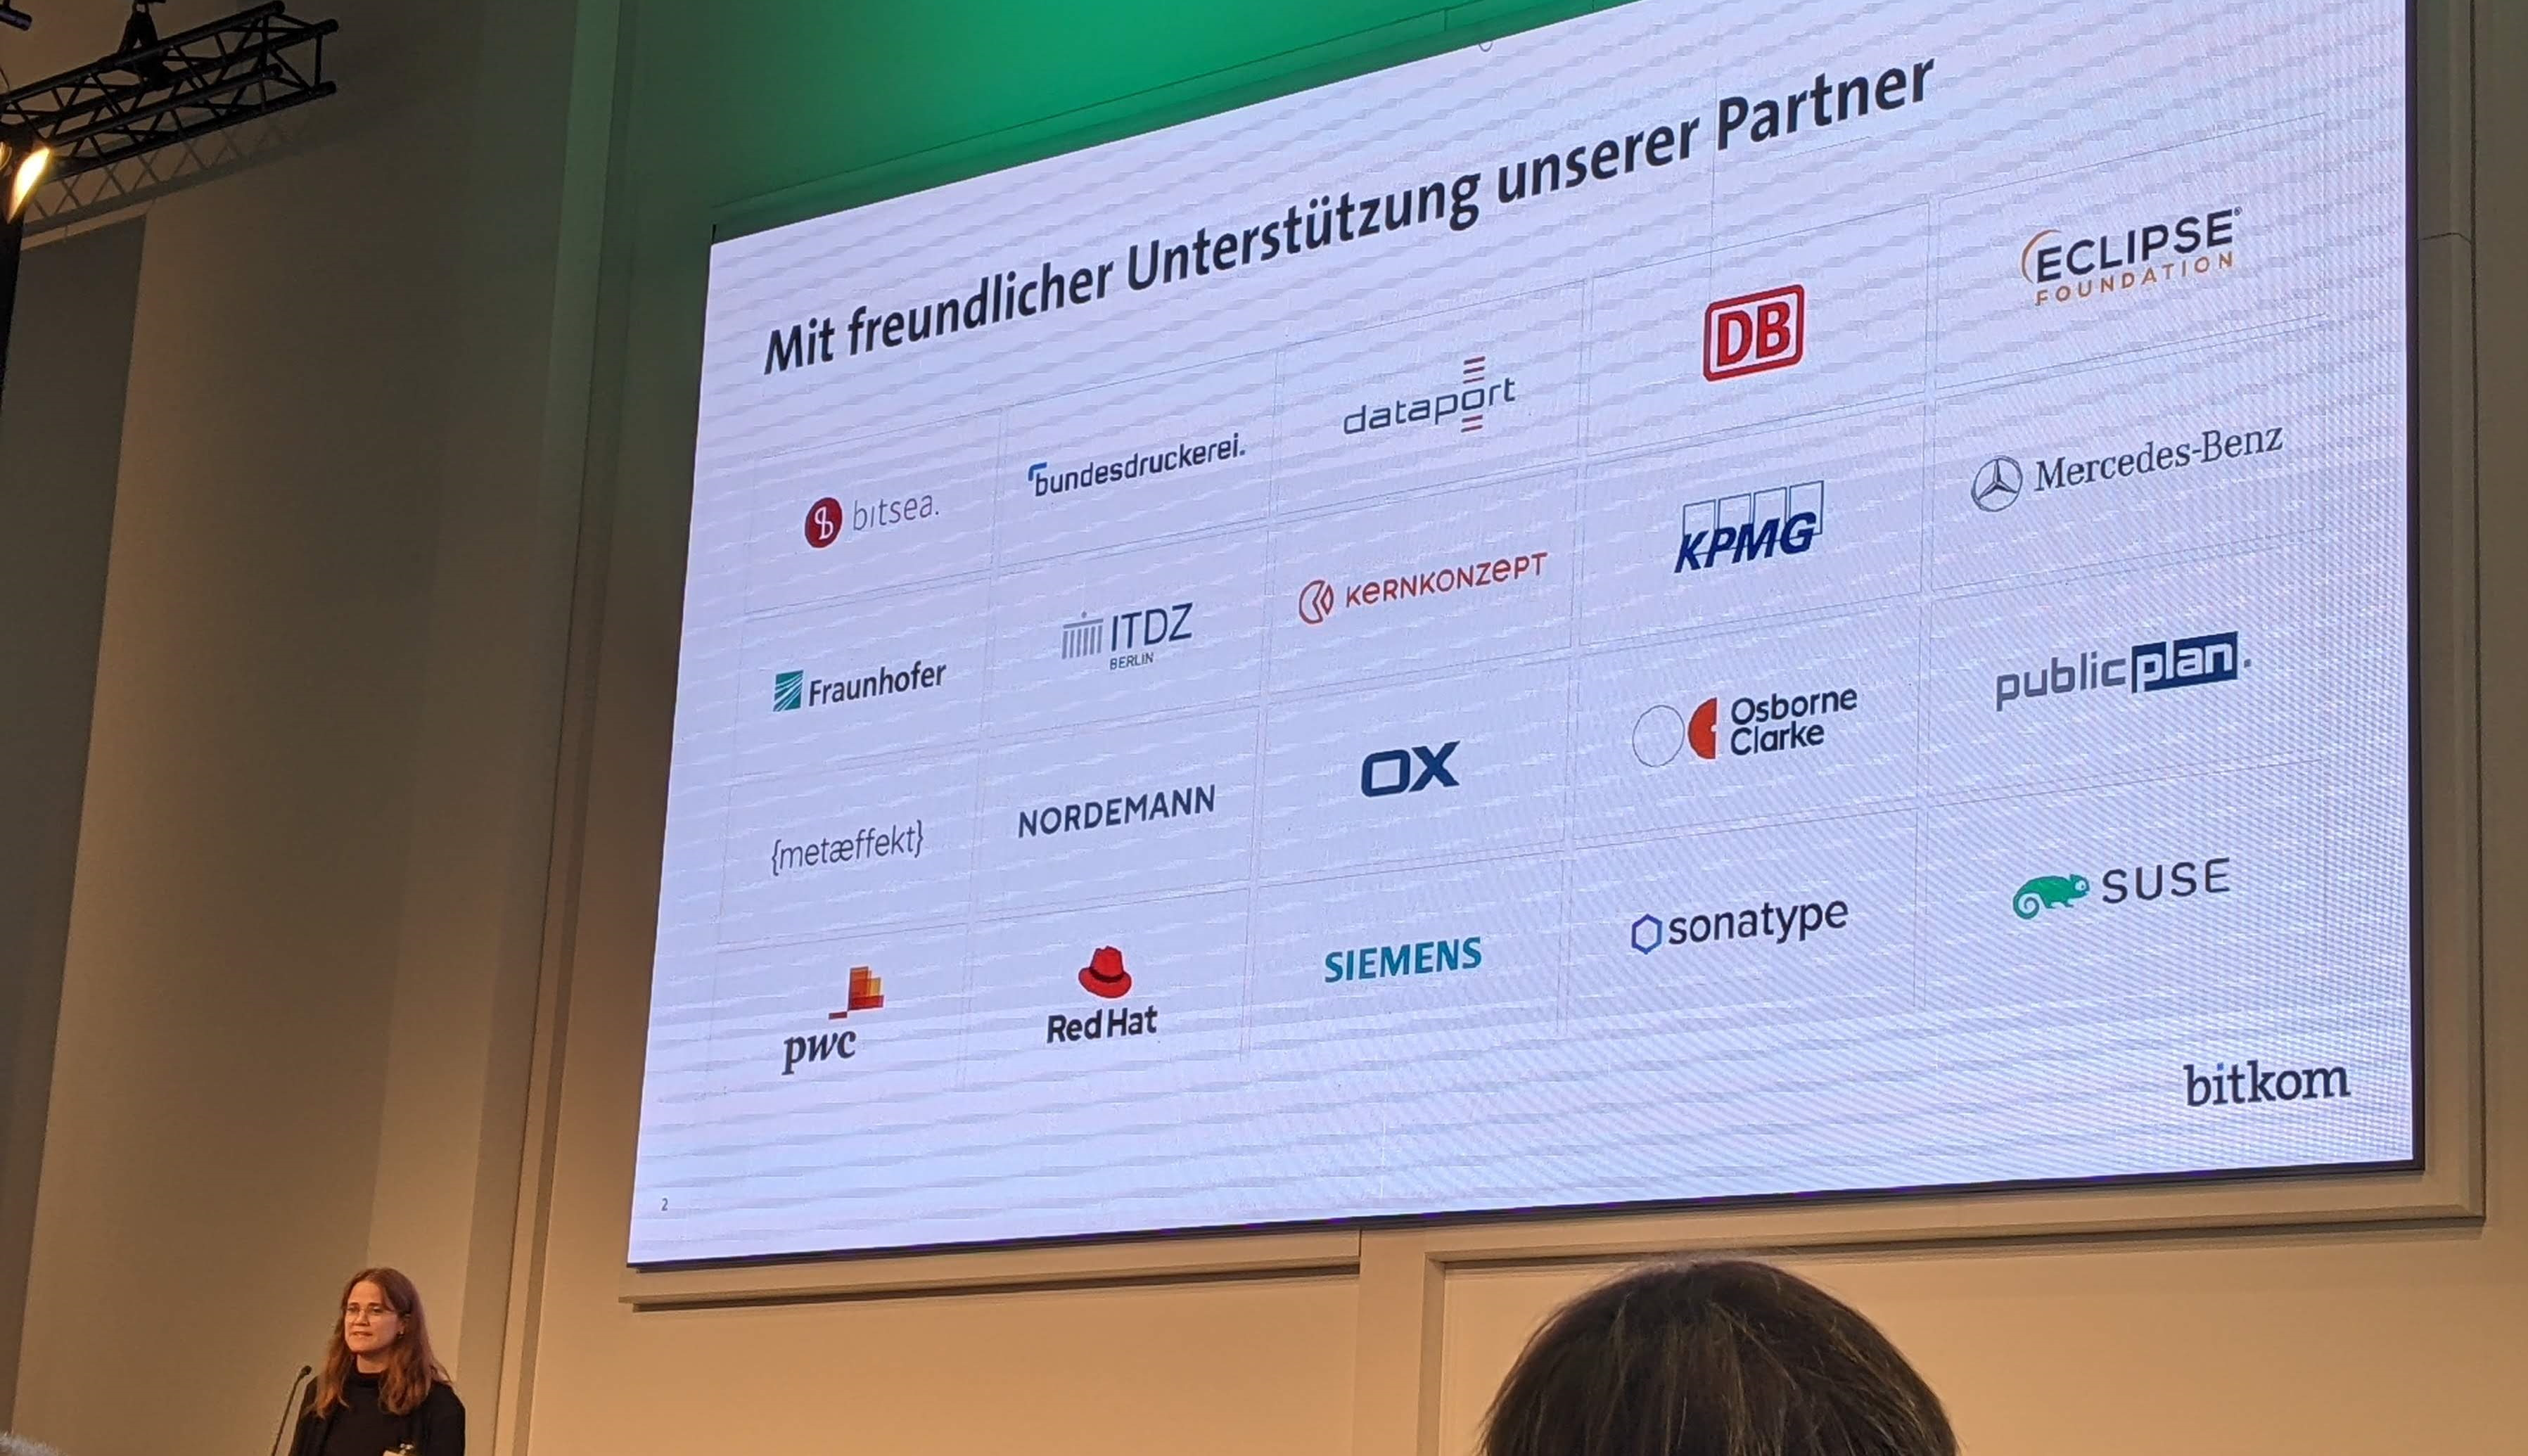
\includegraphics[width=0.8\textwidth, keepaspectratio]{res/img/2023-10-19-ak-os-metaeffekt-sponsor}
    \caption{Die {\metaeffekt} ist links als Sponsor zum OpenSource Monitor aufgeführt}
    \label{fig:foss23-sponsor-metaeffekt}
\end{figure}

Es gab einige bekannte Gesichter vom vorherigen Tag, aber auch einige unserer direkten Kunden waren vertreten, die ich noch nie in Person getroffen hatte.
Außerdem hatte ich die fantastische Chance direkt mit Studenten und Angestellten verschiedener Unterehen zu sprechen.

\sweekdaymarginpar{\weekdayThursdayShort, \weekdayFridayShort}

Die Rückreise am Donnerstag verlief ohne Zwischenfälle, sodass der Freitag wieder der gewöhnliche Arbeitsalltag war.
Eine neue Kundenanforderung erforderte schon wieder meine direkte Aufmerksamkeit:
Einer unserer Download-Prozesse scheitert in ihrer Konfiguration, da der verwendete git-Befehl die konfigurierte Proxy-Informationen bislang scheinbar ignoriert.
Um das zu lösen, kann Git sowohl über Umgebungsvariablen konfiguriert werden, als auch über einen Konfigurationsparameter im Befehlsaufruf.
Ich habe mich für die Umgebungsvariablen entschieden, die ich in der Prozess-Session, die über Java geöffnet wird, mit den Proxy-Informationen setzen kann.

Ein persönliches Highlight war diesen Freitag allerdings noch, dass mein Bruder nun auch Teil des Teams wird.
Über die letzten Tage hat er seine Bewerbung abgeschlossen, wurde angenommen und hat heute noch seinen Arbeitsvertrag unterzeichnet.
Er wird ab sofort die Korrelationsarbeiten des anderen Kollegen übernehmen.
